\documentclass{article}

\usepackage[francais]{babel}
\usepackage[T1]{fontenc}
\usepackage{moreverb}       % verbatim with tab

\usepackage{wrapfig}
\usepackage{graphicx}
\usepackage{geometry}
\geometry{hmargin=2.5cm}
\usepackage{amsmath}
\usepackage{siunitx}

\usepackage{graphicx}
\usepackage{subcaption}
\usepackage{float}
\usepackage{hyperref}
\usepackage{setspace}
\usepackage{xcolor}
\usepackage{pdfpages}
\usepackage{enumitem}
\usepackage{lscape}

\usepackage{fancyhdr}       % en-têtes
\usepackage{lastpage}       % numéro de dernière page

\title{Temps réel}
\date{2021}
\author{Laura Bin}

\pagestyle{fancy}
\renewcommand\headrulewidth{1pt}
\fancyhead[L]{Laura Binacchi}
\fancyhead[C]{Temps réel}
\fancyhead[R]{\today}

\begin{document}
    \pagenumbering{arabic}

    \begin{center}
        \textbf{\LARGE Exercice 3 -- Lecteurs-Écrivains}
    \end{center}

    \paragraph{}
    On va illustrer l'accès à des données partagées dans la sémantique lecteurs/écrivains (les lectures ne sont pas destructrices, contrairement à l'accès en producteur/consommateur).

    \subsection*{Scénario}

    \paragraph{}
    Ici, il y a une seule donnée partagée qui s'appelle Data, utilisée par des threads lecteurs et des threads écrivains. Les threads écrivains incrémentent la variable partagée de différentes valeurs tant que cette variable reste inférieure à une valeur maximum, donnée par VALMAX, alors tous les threads s'arrêtent, aussi bien les lecteurs que les écrivains.

    \paragraph{}
    L'application doit fonctionner de la façon suivante:
    \begin{enumerate}
        \item Le premier lecteur interdit l'accès aux éventuels écrivains suivants, mais pas aux autres lecteurs.
        \item Un écrivain interdit tout autre accès.
        \item Le point 1 peut provoquer la famine pour les écrivains : si un écrivain arrive, il doit attendre la fin du flot des lecteurs avant d'accéder à la ressource.
        \item Pour éviter ce dysfonctionnement, qui peut se traduire par la famine pour les écrivains, l'arrivée d'un écrivain doit bloquer tous les lecteurs suivants. Voici le comportement qui sera adopté : lorsqu'un écrivain se présente, il attend la sortie des lecteurs courants, les lecteurs qui le suivent sont bloqués. Lorsque tous ces lecteurs sont sortis, l'écrivain modifie la donnée, et on sert le (ou les) écrivains(s) qui seraient arrivés entre-temps.
        \item Lorsqu'un écrivain a fini une mise à jour, il donne d'abord accès aux écrivains qui attendent, si il y en a, les lecteurs passeront après. Pour cela, donner une priorité aux threads écrivains afin que l'OS réveille d'abord des écrivains en attente avant des lecteurs en attente (cf \emph{The Little Book of Semaphores}, p. 85, listing 4-23 et 4-24).
        \item Pour que le déroulement soit lisible, implémenter une durée aléatoire de lecture/écriture (sous forme de sleep).
    \end{enumerate}

    \newpage
    \section{Compilation}
    La compilation est réalisée en utilisant cmake via le fichier \emph{CMakeLists.txt} :
    \begin{verbatimtab}
    [1]     cmake_minimum_required(VERSION 3.10)

    [2]     project(project(Exercice3_Lecteurs_Ecrivains VERSION 1.0) VERSION 1.0)

    [3]     set(CMAKE_C_FLAGS "${CMAKE_C_FLAGS} -Wall -Wpedantic -Wextra")

    [4]     include_directories(PUBLIC include)

    [5]     set(SOURCE_FILES
                src/main.c
                src/reader_writer.c
                src/lightswitch.c
                src/data.c)

    [6]     find_package(Threads REQUIRED)

    [7]     add_executable(reader_writer ${SOURCE_FILES})

    [8]     target_link_libraries(reader_writer PRIVATE Threads::Threads)
    \end{verbatimtab}

    \begin{description}
        \item[\texttt{[1]}] version de \texttt{cmake} utilisée
        \item[\texttt{[2]}] nom et version du projet
        \item[\texttt{[3]}] ajout des flags habituels pour l'affichage de tous les warnings
        \item[\texttt{[4]}] le répertoire \emph{include} contient les headers nécessaires à la compilation
        \item[\texttt{[5]}] définition de la variable \texttt{SOURCE\_FILES} contenant les fichiers sources du projet
        \item[\texttt{[6]}] ajout du package pour l'utilisation des threads
        \item[\texttt{[7]}] la compilation des fichiers sources produit l'exécutable \texttt{reader\_writer} 
        \item[\texttt{[8]}] le projet utilise la librairie \texttt{Threads} du package \texttt{Threads}
    \end{description}

    \newpage
    \paragraph{}
    La commande \texttt{cmake -DCMAKE\_C\_FLAGS=-g ..}\footnote{\texttt{-g} permet d'ajouter des informations sur le code source} lancée depuis le sous-répertoire \emph{build} permet de générer le \emph{Makefile} :
    \begin{figure}[H]
        \centering
        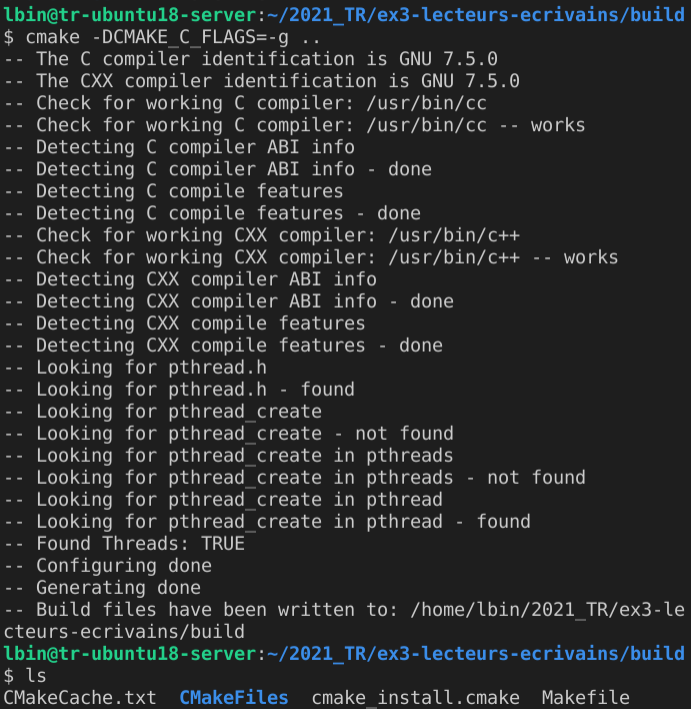
\includegraphics[width=.65\textwidth]{./screenshots/cmake.png}
    \end{figure}

    \paragraph{}
    Par défaut, le \emph{Makefile} est généré en mode debug. Pour le générer en mode release, j'utilise la commande \texttt{cmake -DCMAKE\_BUILD\_TYPE=Release \emph{path}}, où \texttt{\emph{path}} est l'endroit où se trouve le fichier \emph{CMakeLists.txt}.
    
    \newpage
    \paragraph{}
    La commande \texttt{make} permet de compiler le projet à partir du \emph{Makefile} pour produire l'exécutable \emph{reader\_writer} :
    \begin{figure}[H]
        \centering
        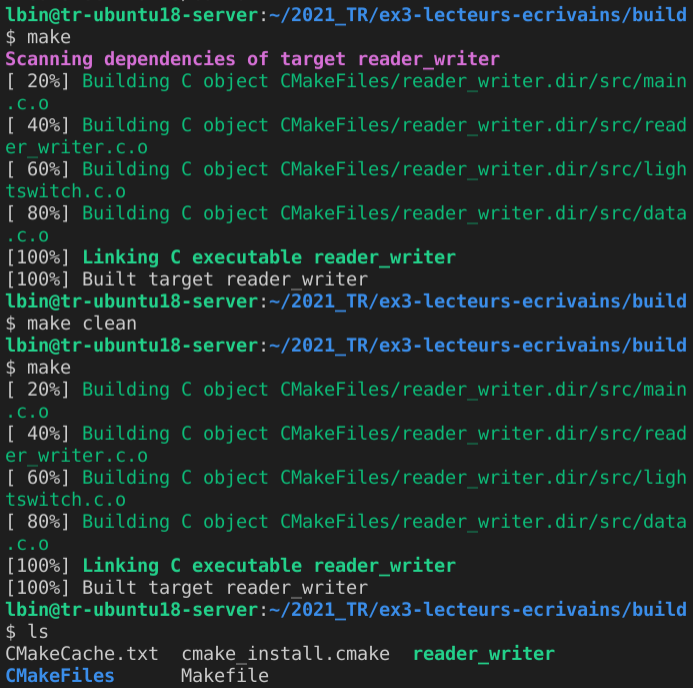
\includegraphics[width=.65\textwidth]{./screenshots/make.png}
    \end{figure}

    \newpage
    \section{Tests}
    \subsection{Cas nominal}
    La programme a été testé avec des temporisations aléatoires plus longues pour les threads lecteurs que pour les threads écrivains :
    \begin{figure}[H]
        \centering
        \begin{subfigure}[b]{.49\textwidth}
            \centering
            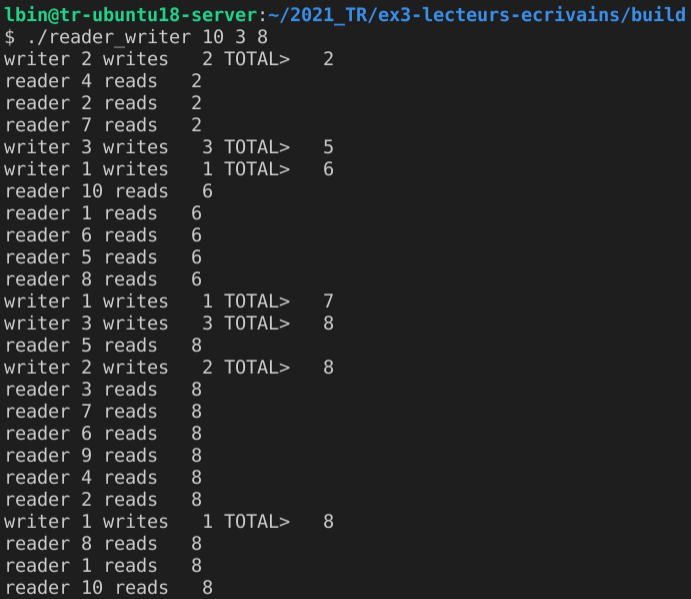
\includegraphics[width=\textwidth]{./screenshots/test1.png}
        \end{subfigure}
        \begin{subfigure}[b]{.49\textwidth}
            \centering
            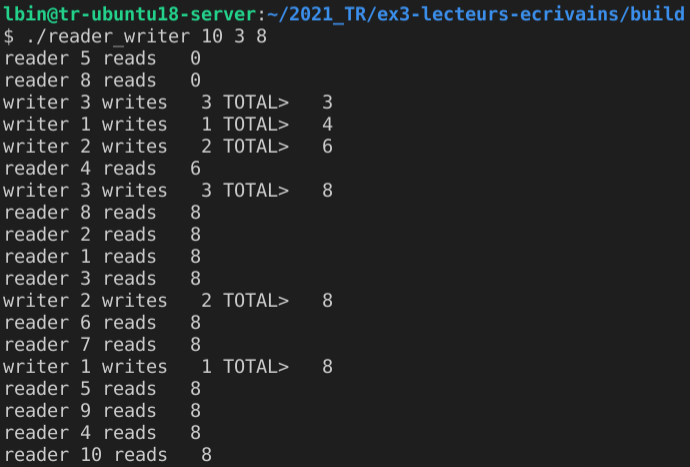
\includegraphics[width=\textwidth]{./screenshots/test2.png}
        \end{subfigure}
    \end{figure}

    \paragraph{}
    Le lightswitch des lecteur et celui des écrivains permettent bien de laisser passer plusieurs lecteurs ou plusieurs écrivains dans la zone d'accès à la donnée :
    \begin{figure}[H]
        \centering
        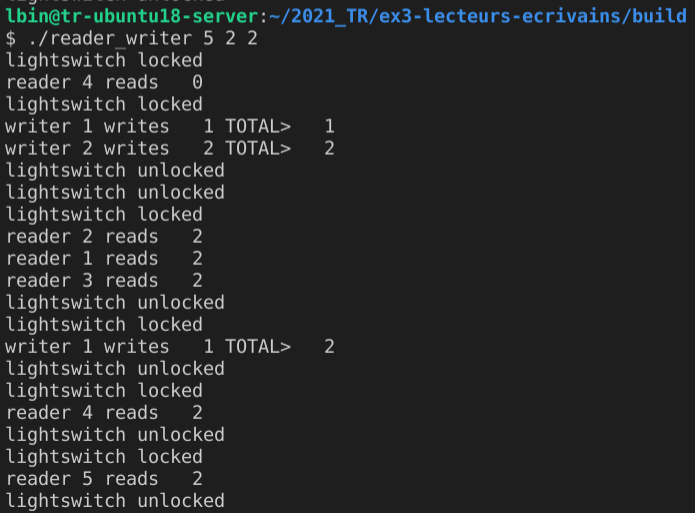
\includegraphics[width=.6\textwidth]{./screenshots/test_lightswitch.png}
    \end{figure}

    \subsection{Cas d'erreur}
    \paragraph{}
    Le programme attend en paramètres le nombre de threads lecteurs, de threads écrivains et la valeur maximale de la donnée.
    \begin{figure}[H]
        \centering
        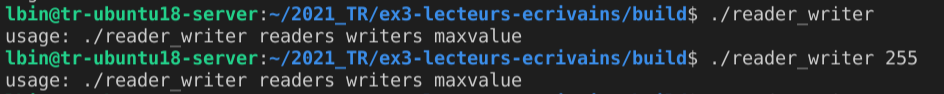
\includegraphics[width=.8\textwidth]{./screenshots/invalid_args.png}
    \end{figure}

    \paragraph{}
    Le nombre de \emph{readers} (threads de lecture de la donnée partagée) doit être supérieur à 0:
    \begin{figure}[H]
        \centering
        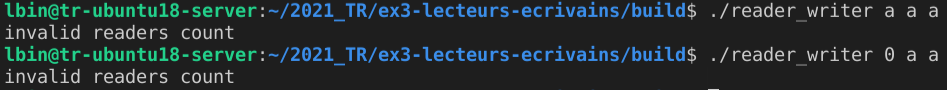
\includegraphics[width=.8\textwidth]{./screenshots/invalid_readers_count.png}
    \end{figure}

    \paragraph{}
    Le nombre de \emph{writers} (threads d'incrémentation de la donnée partagée) doit être supérieur à 0:
    \begin{figure}[H]
        \centering
        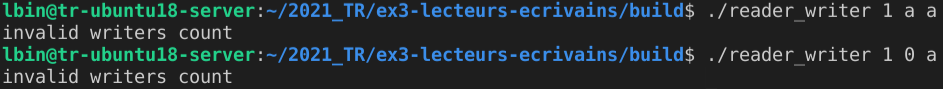
\includegraphics[width=.8\textwidth]{./screenshots/invalid_writers_count.png}
    \end{figure}

    \paragraph{}
    La valeur maximale de la donnée doit être supérieure à 0:
    \begin{figure}[H]
        \centering
        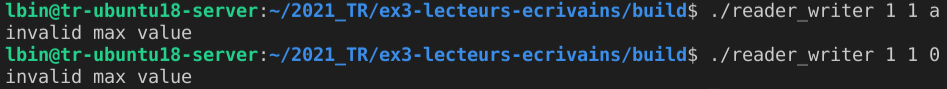
\includegraphics[width=.8\textwidth]{./screenshots/invalid_max_value.png}
    \end{figure}

    \paragraph{}
    Des valeurs trop grandes stoppent également le programme:
    La valeur maximale de la donnée doit être supérieure à 0:
    \begin{figure}[H]
        \centering
        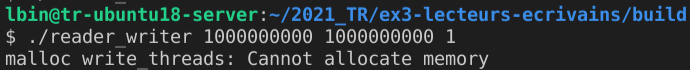
\includegraphics[width=.6\textwidth]{./screenshots/malloc_error.png}
    \end{figure}

    \newpage
    \subsection{Valgrind}
    \paragraph{}
    Le test du programme avec \emph{valgrind} permet de voir qu'il n'y a pas de fuite mémoire (tous les espaces mémoire alloués ont bien été libérés) :
    \begin{figure}[H]
        \centering
        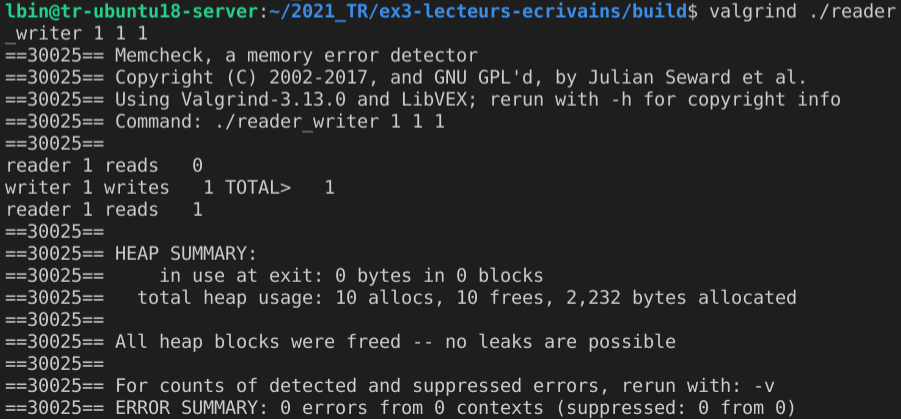
\includegraphics[width=.8\textwidth]{./screenshots/test_valgrind.png}
    \end{figure}
\end{document}
